% !TEX root = ../../thesis.tex
    
%**************************************************************
% Methodology
%*************************************************************
\chapter{Metodologie di Analisi}
    Ai fini di valutare le performance delle soluzioni dei vari modelli applicati sul dataset che rappresenta la latenza media 
    delle richieste a servizi fatti a Infostud, viene proposto l'utilizzo di tre principali approcci metodologici per 
    l'analisi atta all'individuazione di anomalie nel dataset accademico. Le soluzioni verranno analizzate 
    in virtù delle etichette dapprima esistenti sul dataset:
    \begin{enumerate}
        \item \textbf{Approccio Statistico (Statistical-based):} L'approccio statistico si basa sulla tradizionale 
              statistica dei dati. In particolare ARMA\cite{arma}, il modello utilizzato per fare inferenza sulle anomalie 
              del prezioso dataset di Infostud, modella le relazioni temporali nei dati attraverso l'uso dell'autoregressione 
              e della media mobile, metodi adatti al fine di modellare le relazioni temporali nei dati; il modello 
              identifica tendenze e autocorrelazioni nelle metriche applicate.
        \item \textbf{Approccio di Apprendimento Automatico (Machine Learning-based):} Nell'ambito dell'apprendimento automatico, 
              è stato scelto l'approccio basato sulle Support Vector Machine (SVM). In particolare, la Support Vector 
              Machine a classe singola (OC-SVM\cite{ocsvm}), un algoritmo che si concentra sull'identificazione di 
              dati fuori dal normale comportamento in grado di tracciare confini decisionali creando due regioni che 
              discriminano, nel caso in questione, le anomalie dalle non anomalie.
        \item \textbf{Approccio di Apprendimento Profondo (Deep Learning-based):} L'apprendimento profondo è particolarmente 
              efficace nell'affrontare problemi di analisi di dati complessi, come le serie temporali.  
              Questo approccio vede applicati due modelli molto recenti: Telemanom\cite{telemanom} e Multi-Scale Convolutional 
              Recurrent Encoder-Decoder (MSCRED\cite{mscred}); entrambi sono modelli basati su reti neurali e sono 
              progettati con lo specifico obiettivo di individuazione delle anomalie in dati multivariati. 
    \end{enumerate}

    Ciascuno di questi approcci contribuisce in modo significativo all'analisi del dataset indispensabile per tutta 
    la comunità Sapienza, fornendo una varietà di strumenti e metodi per esplorare, valutare e interpretare le 
    informazioni contenute nei dati di Infostud. Nel corso di questo capitolo, verranno esaminate in dettaglio 
    le soluzioni di ciascuno dei modelli presi in considerazione.

    \section{Approccio Statistico (Statistical-based)}
        %**************************************************************
% ARMA
%**************************************************************

\subsection{Auto Regressive Moving Average}
    In questa sezione esploriamo l'uso del modello univariato ARMA\cite{arma} 
    (Auto Regressive Moving Average) come 
    modello di riferimento che adotta un approccio statistico per valutare e confrontare l'efficacia del modello MSCRED\cite{mscred}.
    La scelta del modello ARMA è stata motivata principalmente dalla sua 
    utilizzazione da parte dei ricercatori di MSCRED per valutare le prestazioni di quest'ultimo. In generale, 
    ARMA è un modello ben consolidato e ampiamente utilizzato nella letteratura grazie alla sua semplice 
    implementazione e intuitività.

    Tuttavia, la sua semplicità ha un costo: il modello non è in grado di catturare l'intercorrelazione 
    tra i segnali perché è monovariato per natura. 
    Nell'esperimento presentato, per adattarsi alla natura monovariata del modello, è stato selezionato il
    segnale meno vuoto dal dataset di Infostud descritto nel \hyperref[cap2]{Capitolo 2}, ovvero il segnale con
    il minor numero, solo dieci, di valori nulli, avendo quindi a disposizione un totale di 48327 osservazioni.
    Il segnale interessato rappresenta la latenza media delle richieste di login a InfoSapienza.


    \paragraph{Intuizione} ARMA, nelle serie temporali, è utilizzato principalmente per la previsione di dati, ma 
    può essere usato anche per la rilevazione di anomalie. In linea generale, data una previsione di ARMA, i punti 
    in cui la previsione si discosta maggiormente rispetto ai punti originali vengono considerati anomalie.

    Più in dettaglio, ARMA effettua una certa previsione $P$ basata sui dati di training. Tale previsione viene 
    confrontata con i valori ground-truth $G$ calcolando i residui $P-G$. Attraverso l'iperparametro $t$ 
    vengono calcolati i confini decisionali $c^-, c^+$. ogni punto $i$ è valutato come anomalia se $P_i-G_i \notin [c^-, c^+]$,
    e non è valutato come tale altrimenti. 
    I confini decisionali $c^-, c^+$ sono ottenuti come segue: siano $\mu$ la media dei valori dell'unico segnale
    del dataset e sia $\sigma$ la sua deviazione standard: $c^+ = \mu + t^*\cdot\sigma, c^- = \mu - t^*\cdot\sigma$



    \paragraph{Dataset}Il dataset di Infostud è stato suddiviso in tre insiemi: training, validation e
    test, con percentuali rispettivamente pari a $0.5, 0.182, 0.318$. Allo scopo di 
    garantire una distribuzione accettabile delle anomalie nei tre insiemi, questa suddivisione atipica è stata 
    necessaria a causa della natura delle anomalie nel dataset, che sono principalmente di tipo collettivo 
    e quindi vicine tra loro sia nel tempo che nello spazio.
    Nel dataset, come già annunciato, è stato preso in considerazione un solo segnale, quello che rappresenta 
    la latenza media delle richieste di login effettuate a InfoSapienza, i cui dieci punti originariamente nulli 
    sono stati rimossi.
    Nella \hyperref[tab:dataset-arma]{Tabella 3.1.} sono riportate le informazioni in dettaglio della suddivisione 
    del dataset e nella \hyperref[fig:dataset-arma]{Figura 3.1.} è illustrato il dataset.

    \begin{table}[H]
        \centering
        \caption{Statistiche dataset ARMA (latenza media delle richieste di login).}
        \begin{tabular}{lccc}
            \toprule
            \textbf{Dataset} & \textbf{Indice di split} & \textbf{\# punti} & \textbf{Anomalie (\%)} \\
            \midrule
            \textbf{Training} & 0.5 & 24163 & 2.01 \% \\
            \textbf{Validation} & 0.182 & 8796 & 8.59 \% \\
            \textbf{Testing} & 0.318 & 15368 & 9.59 \% \\
            \bottomrule
        \end{tabular}
        \label{tab:dataset-arma}
    \end{table}

    \begin{figure}[H]
        \centering
        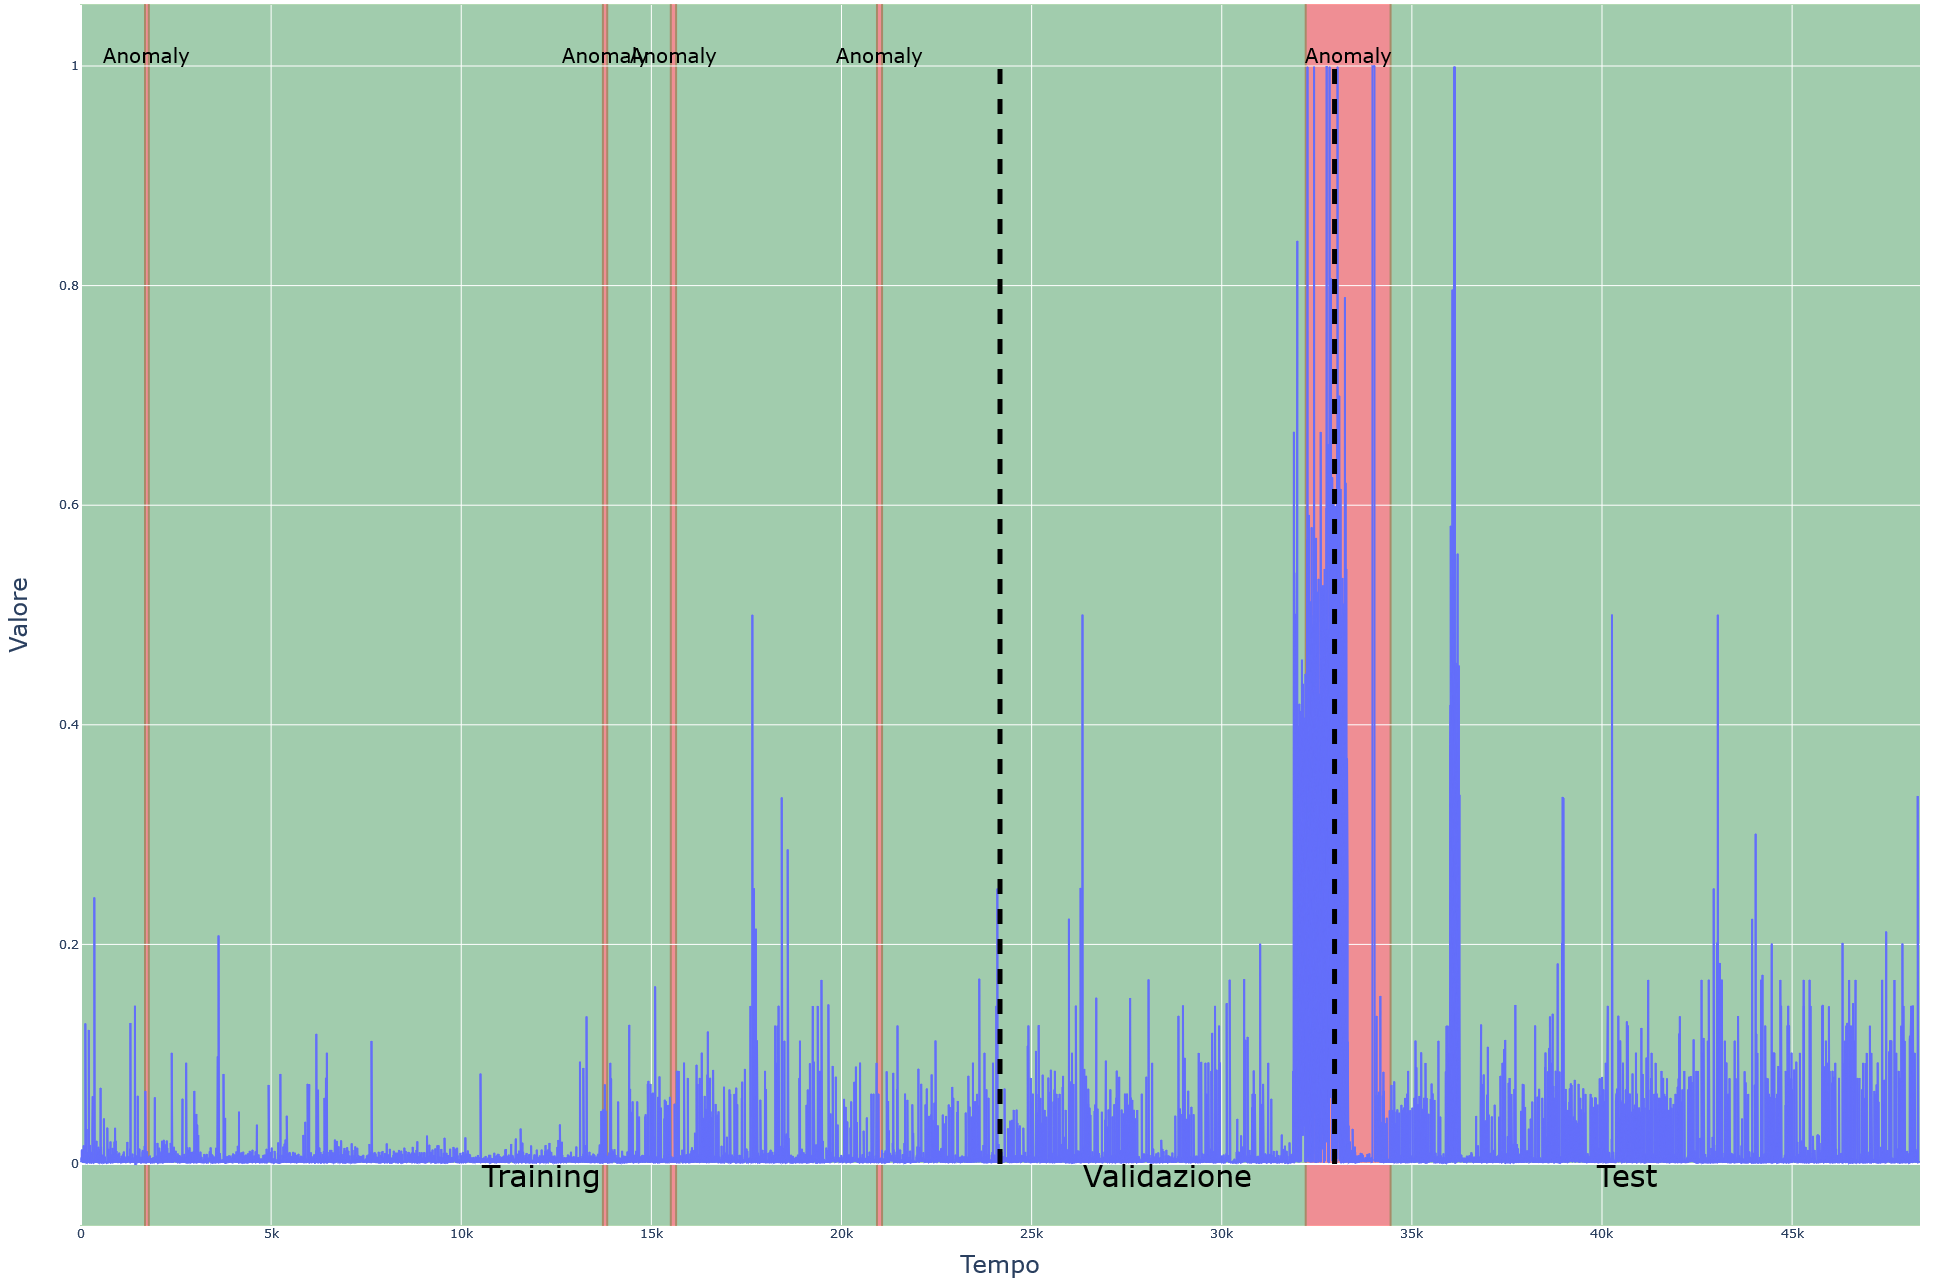
\includegraphics[width=0.6\textwidth]{./input/chapters/models/figs/arma-dataset.png}
        \caption{Dataset delle latenze medie alle richieste di login nel periodo 23 maggio - 22 giugno 2020. 
        Le bande rosse rappresentano le anomalie ground-truth, mentre quelle verdi i periodi non anomali. 
        Le linee tratteggiate delimitano il dataset di training da quello di validazione e quello di validazione dal test.}
        \label{fig:dataset-arma}
    \end{figure}

    \paragraph{Iperparametri} ARMA, in generale, presenta due iperparametri $p,q$. $p$ rappresenta l'ordine 
    dell'autoregressione nel modello ARMA. L'autoregressione si riferisce al fatto che il valore corrente 
    della serie temporale dipende dai valori passati della stessa serie temporale, in sintesi $p$ indica 
    quanti periodi temporali passati vengono utilizzati per predire il valore corrente ed è l'iperparametro 
    che fa sì che ARMA possa catturare le dipendenze temporali nella serie temporale. $q$, invece, 
    rappresenta l'ordine della media mobile nel modello. Essa indica che il valore della corrente serie 
    temporale dipende dai valori passati dei residui, ovvero degli errori previsionali, del modello stesso.
    Intuitivamente, $q$ indica quanti periodi temporali passati degli errori previsionali vengono utilizzati per 
    predire il valore corrente.

    Ai fini dell'anomaly detection, ARMA presenta anche un terzo iperparametro $t$ che, nel caso degli studi effettuati,
    è atto a creare i confini decisionali dei punti non anomali e, dualmente, anomali, definendo la sensibilità 
    del modello. 

    Per la scelta degli iperparametri è stata effettuata una grid-search di 30 epoche su $p$, $q$ e $t$  al fine di 
    individuare la combinazione che massimizzasse lo score F1, metrica illustrata nella \hyperref[f1-score]{Sottosezione 4.1.3}, 
    sul dataset di validation attraverso il training sul train set.

    Formalmente, siano $\mathbf{Tr}, \mathbf{Va}$ i dataset utilizzati per il training e
    per il validation rispettivamente, e sia $\text{ARMA}_\mathbf{X}^\mathbf{Y}$ un modello ARMA addestrato su 
    $\mathbf{X}$ che effettua previsioni nei punti $\mathbf{Y}$ e sia $T_{10}$ uno spazio lineare composto da 
    elementi equidistanti $t_i$ tali che $t_i \in [0.1, 5.0] \forall i \in [10]$:
    \begin{equation}
    \label{eq:arma-problem}
    \begin{aligned}
        & p^*, q^*, t^* = \max_{p, q, t} F1(\text{ARMA}_\mathbf{Tr}^\mathbf{Va}(p, q, t)) \\
        & \text{con il vincolo} \quad p, q \in [30], t \in T_{10}
    \end{aligned}
    \end{equation}


    \paragraph{Soluzione} \hyperref[eq:arma-problem]{L'equazione 3.1}  è stata soddisfatta dai seguenti:
    \begin{itemize}
        \item $p^* = 20$
        \item $q^* = 8$
        \item $t^* = 0.644$
    \end{itemize}

    Poiché l'insieme di validazione era necessario solo ai fini della ricerca degli iperparametri, è 
    stato successivamente accorpato al dataset di training. Dopo l'addestramento del modello sul nuovo dataset 
    con gli iperparametri che hanno generato una soluzione ottimale sul validation, sono state effettuate 
    le previsioni della serie temporale di test, mostrate nella \hyperref[fig:arma-sol]{Figura 3.2.}


    \begin{figure*}[h]
        \centering
        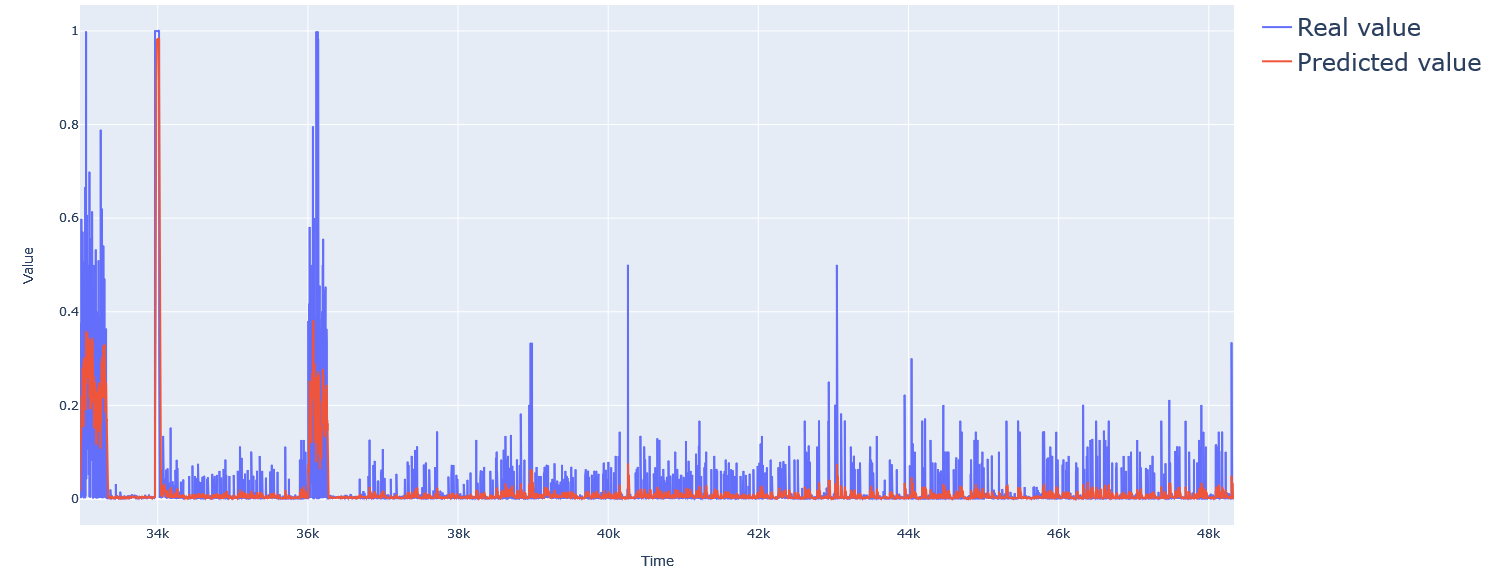
\includegraphics[width=0.7\textwidth]{./input/chapters/models/figs/arma-sol.png}
        \caption{Confronto della previsione del modello e le osservazioni originali sull'insieme di test.}
        \label{fig:arma-sol}
    \end{figure*}

    È evidente che il modello è in grado di prevedere l'andamento generale della serie temporale per la maggior
    parte del dataset. Tuttavia, in alcune aree, il modello presenta una performance inferiore rispetto ad altre.
    Queste aree saranno cruciali per la classificazione dei punti come anomali o non anomali.

    Sulla base delle previsioni $P$, sono stati calcolati i residui rispetto al test set $P-G$ e valutati come punti 
    anomali quelli che soddisfano $p_i-g_i \notin [c^-, c^+] | p_i \in P, g_i \in G$. I residui sono illustrati nella \hyperref[fig:residuals]{Figura 3.3.}

    I punti all'interno dell'intervallo definito dai confini inferiore e superiore non sono considerati anomali. 
    Tra questi punti ci sono quelli blu, che non sono anomalie e che il modello non ha considerato come tali
    (True Negatives), e quelli viola, che il modello ha erroneamente classificato come non anomalie (False Negatives).

    Possiamo inoltre osservare che svariati punti in verde sono sono stati correttamente classificati come anomalie
    (True Positives), ma sono presenti anche molti punti rossi, ovvero quelli che il modello ha erroneamente 
    considerato anomalie (False Positives). 

    \begin{figure}[H]
        \centering
        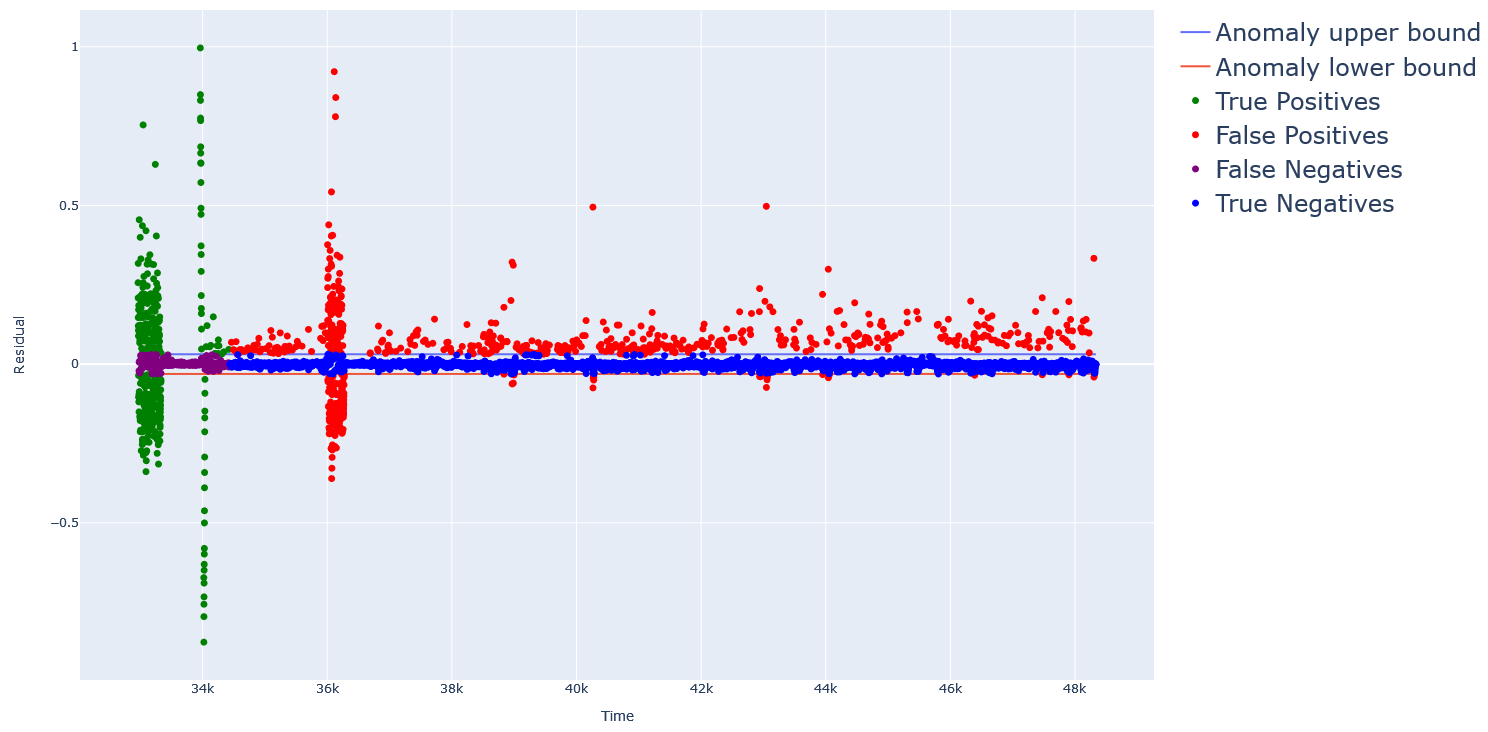
\includegraphics[width=0.7\textwidth]{./input/chapters/models/figs/arma-residuals.png}
        \caption{I residui del modello ARMA nel test set con i confini decisionali che discriminano la previsione delle 
        anomalie e le non anomalie.}
        \label{fig:residuals}
    \end{figure}

    \section{Approccio di Apprendimento Automatico (Machine Learning-based)}
        %**************************************************************
% ocsvm
%**************************************************************
\subsection{One-Class Support Vector Machine}
    In questa sottosezione, esaminiamo il modello basato sull'apprendimento automatico One-Class Support Vector 
    Machine\cite{ocsvm} (OC-SVM) come altro punto di riferimento per valutare le prestazioni del modello 
    MSCRED\cite{mscred}. La scelta del modello OC-SVM è motivata dalla sua ampia utilizzazione nella 
    letteratura di riferimento e dal suo impiego da parte dei ricercatori di MSCRED per il confronto delle 
    prestazioni. In generale, gli algoritmi di tipologia Support Vector Machine sono noti per offrire buone 
    prestazioni in diversi contesti. Tuttavia, tendono a soffrire quando si tratta di classificazione di 
    anomalie, poiché le anomalie costituiscono solitamente una piccola parte del dataset, creando uno 
    sbilanciamento tra le classi.

    \paragraph{Intuizione} OC-SVM, come gli altri algoritmi della famiglia SVM, opera tracciando confini 
    decisionali tra i dati. Nell'ambito della rilevazione delle anomalie, questo si traduce nella definizione 
    di un iperpiano che separa i punti considerati anomali da quelli considerati non anomali.

    \paragraph{Dataset} Nell'esperimento è stato suddiviso il dataset di riferimento negli insiemi di training, 
    validation e test con le stesse percentuali utilizzate per ARMA, ovvero $0.5, 0.182, 0.318$ rispettivamente. 
    La \hyperref[tab:dataset-ocsvm]{Tabella 3.2.} mostra la percentuale di anomalie in ciascun 
    sottoinsieme del dataset originale, mentre nella \hyperref[fig:dataset-div1]{Figura 3.4.} viene
    evidenziato il dataset partizionato.


    \begin{table}[H]
        \centering
        \caption{Statistiche dataset OC-SVM.}
        \begin{tabular}{lccc}
            \toprule
            \textbf{Dataset} & \textbf{Indice di suddivisione} & \textbf{\# punti} & \textbf{Anomalie (\%)} \\
            \toprule
            \textbf{Training}   & 0.5   &  24168 & 2.01\% \\
            \textbf{Validation} & 0.182 &  8797  & 8.60\% \\
            \textbf{Testing}    & 0.318 &  15372 & 9.59\% \\
            \bottomrule
        \end{tabular}
        \label{tab:dataset-ocsvm}
    \end{table}

    \begin{figure}[H]
        \centering
        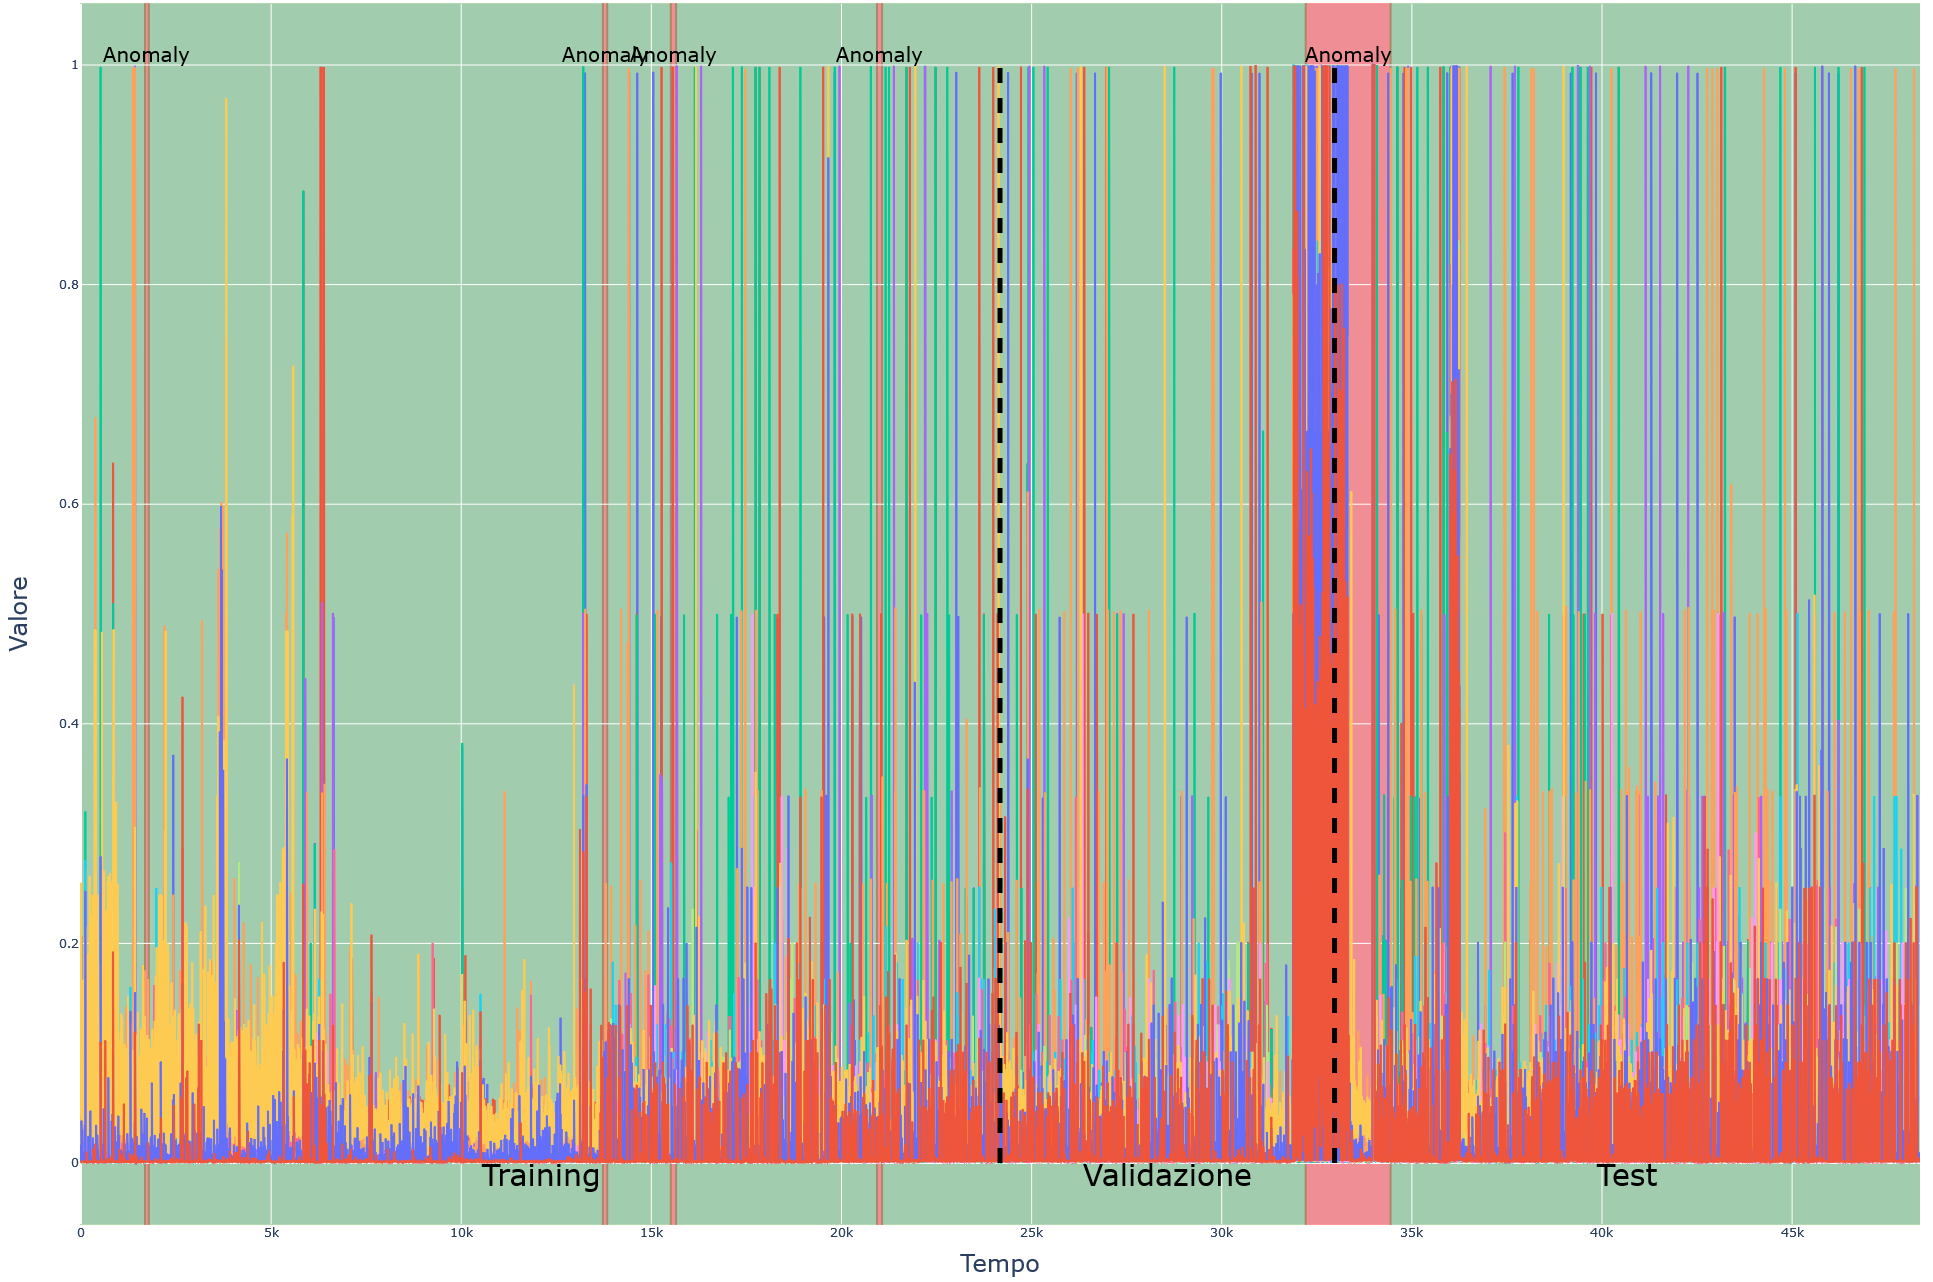
\includegraphics[width=0.5\textwidth]{./input/chapters/models/figs/dataset_div1.png}
        \caption{Suddivisione dataset negli insiemi di training, validation e test. Le due linee 
        tratteggiate rappresentano, da sinistra a destra rispettivamente la suddivisione tra l'insieme di training e 
        validazione e tra l'insieme di validazione e test.}
        \label{fig:dataset-div1}
    \end{figure}


    \begin{table}[H]
        \centering
        \caption{Valori candidati per gli iperparametri.}
        \begin{tabular}{lccc}
            \toprule
            \textbf{Iperparametro} & \textbf{Candidati} \\
            \toprule
            $\nu$ & 0.03, 0.1, 0.25, 0.5, 0.9 \\
            \midrule
            Kernel & linear, poly, rbf, sigmoid \\
            \bottomrule
        \end{tabular}
        \label{tab:iperparametri-candidati}
    \end{table}

        \paragraph{Iperparametri} Gli iperparametri $\nu$ e il tipo di kernel sono stati trovati effettuando una 
        "grid-search" partendo 
        da un insieme di candidati per entrambi gli iperparametri illustrati nella 
        \hyperref[tab:iperparametri-candidati]{Tabella 3.3.} La combinazione di valori $(\nu^*, \text{Kernel}^*)$ che 
        ha massimizzato lo score F1 sul validation set è stata scelta come configurazione ottimale.

        Formalmente, siano $\mathbf{Tr}, \mathbf{Va}$ i dataset utilizzati per il training e
        per il validation rispettivamente e sia $\text{OC-SVM}_\mathbf{X}^\mathbf{Y}$ un modello OC-SVM addestrato
        su $\mathbf{X}$ che effettua previsioni sulle etichette dei punti $\mathbf{Y}$ e sia $K$ l'insieme dei 
        possibili valori che può assumere il kernel, ossia $K=\{\text{linear}, \text{poly}, \text{rbf}, \text{sigmoid}\}$:


    \begin{equation}
        \label{eq:ocsvm-problem}
        \begin{aligned}
            & \nu^*, \text{Kernel}^* = \max_{\nu, \text{Kernel}} F1(\text{OC-SVM}_\mathbf{Tr}^\mathbf{Va}(\nu, \text{Kernel})) \\
            & \text{con il vincolo} \quad \nu \in [0.03, 0.1, 0.25, 0.5, 0.9], \text{Kernel} \in K
        \end{aligned}
    \end{equation}
        
        \paragraph{Soluzione} \hyperref[eq:ocsvm-problem]{L'equazione 3.2}  è stata soddisfatta dai seguenti valori:
        \begin{itemize}
            \item $\nu^* = 0.9$
            \item Kernel$^* = \text{sigmoid}$
        \end{itemize}

        Dopo aver utilizzato l'insieme di validazione esclusivamente per l'ottimizzazione degli iperparametri, 
        è stato poi unito al dataset di addestramento. Successivamente, il modello è stato addestrato sul nuovo
        dataset combinato, utilizzando gli iperparametri che hanno prodotto una soluzione ottimale durante la fase di 
        convalida. In \hyperref[fig:ocsvm-sol]{Figura 3.5.} viene mostrata la 
        soluzione dopo l'applicazione di PCA per fornire una rappresentazione ai primi tre componenti principali.
        
        \begin{figure}[H]
            \centering
            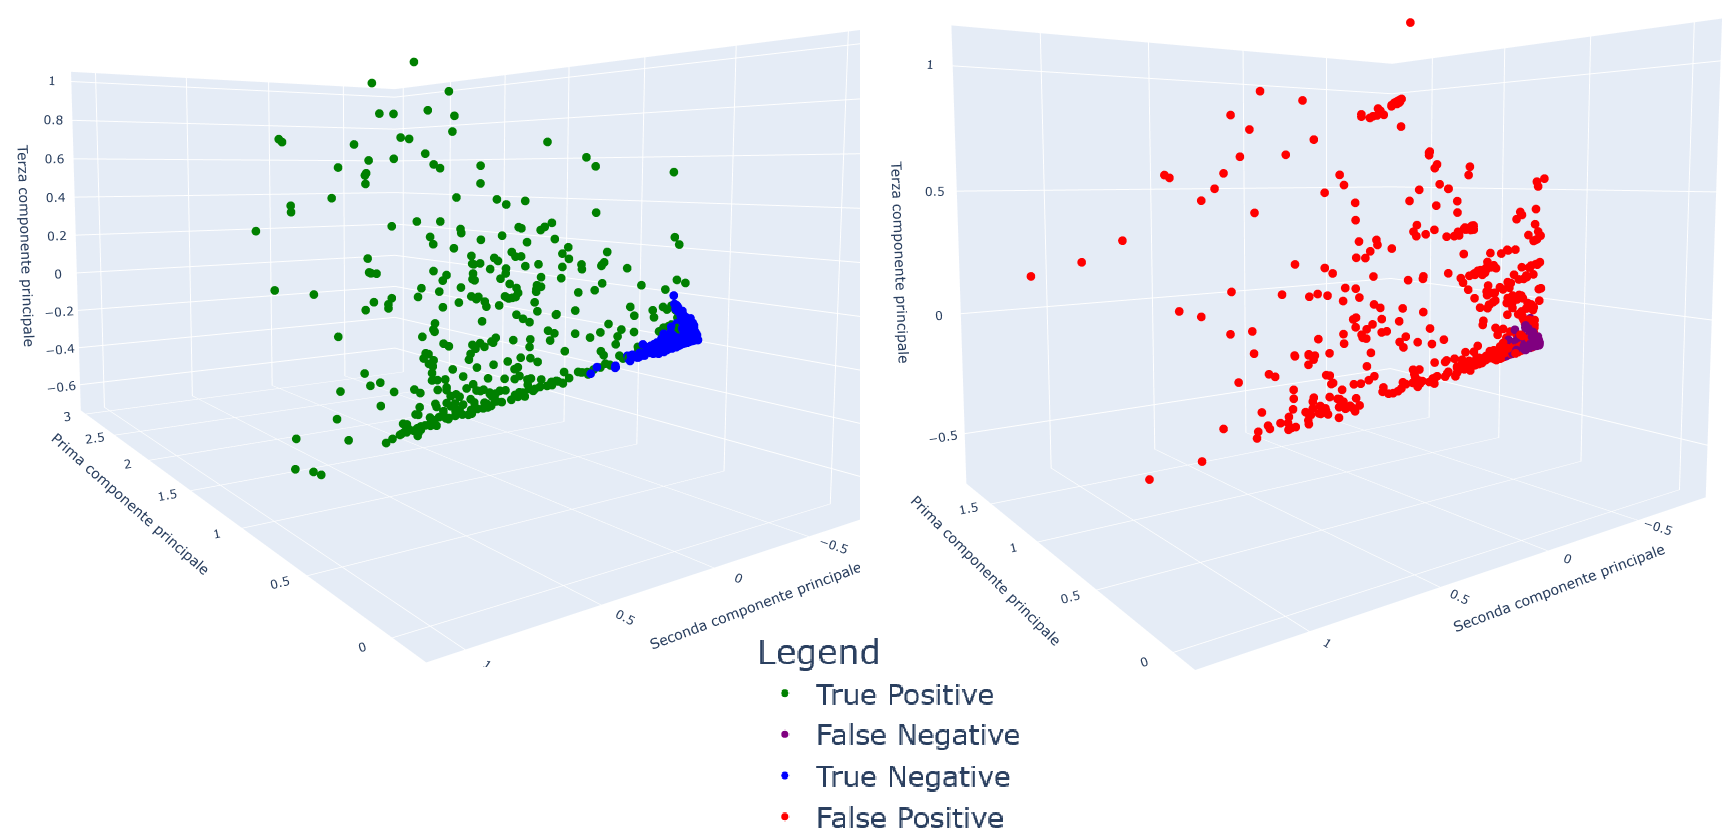
\includegraphics[width=0.7\textwidth]{./input/chapters/models/figs/ocsvm-sol.png}
            \caption{\small
                Soluzione del modello OC-SVM dopo l'applicazione di PCA ai primi tre 
                componenti principali, garantendo una rappresentazione visibile rispetto a quella 
                originale a dodici dimensioni. A sinistra sono rappresentate le previsioni corrette
                (TP, TN), mentre a destra quelle errate (FP, FN).
            }
            \label{fig:ocsvm-sol}
        \end{figure}

        I risultati mostrano chiaramente che il modello ha prestazioni scarse sul dataset di test. 
        I punti verdi a sinistra della \hyperref[fig:ocsvm-sol]{Figura 3.5.} sono quelli classificati correttamente 
        come anomalie (True Positives) e quelli blu sono quelli classificati correttamente come non anomali (True Negatives). 
        Tuttavia, molti punti sono stati classificati in modo errato, come evidenziato a destra nella stessa figura. 
        I punti viola rappresentano le anomalie erroneamente classificate come normali (False Negatives), 
        mentre i punti rossi sono i punti normali erroneamente classificati come anomalie (False Positives).  
        


    \section{Approccio di Apprendimento Profondo (Deep Learning-based)}
          %**************************************************************
% Telemanom
%**************************************************************

\subsection{Telemanom} \label{sez-telemanom}
    Telemanom\cite{telemanom} è una tecnica di rilevazione di anomalie sviluppata dai ricercatori della Nasa nel 2018 
    ai fini dell'anomaly detection su stazioni e veicoli spaziali. Il modello è stato applicato dai ricercatori sui 
    dati telemetrici dei satelliti e del rover Curiosity e, come MSCRED\cite{mscred}, utilizza reti neurali 
    Long-Short Term Memory (LSTM\cite{convlstm}).

    La scelta di utilizzare Telemanom in questa ricerca si è basata sulla necessità di confrontare MSCRED con un modello 
    più recente che sfrutta tecniche avanzate focalizzate sull'apprendimento profondo, concentrandosi esclusivamente 
    sulla rilevazione delle anomalie.

    Il modello nasce come miglioramento ai vecchi sistemi di anomaly detection per l'attrezzatura spaziale 
    che, in generale, erano semplicemente basati su valori precisi e predeterminati che, una volta superati, facevano sì che venissero
    attivate le misure di sicurezza opportune. Telemanom è stato progettato tenendo presente che i dati vivono in un 
    contesto non supervisionato ed è in grado di osservare segnali multipli e analizzare se un certo canale (segnale)
    si trova in uno stato anomalo o meno individualmente dagli altri segnali. Questo permette di tracciare più facilmente 
    le cause dell'anomalia. Per cui Telemanom tratta un contesto ancora più complesso rispetto a quello in cui vive InfoSapienza, 
    dove le anomalie sono globali per tutti i segnali.

    \paragraph{Intuizione} Telemanom effettua previsioni creando un modello distinto per ciascun canale di telemetria,
    questo significa che ogni canale viene trattato in modo indipendente per la previsione. Il modello
    viene addestrato per predire un certo numero di valori futuri per ciascun canale di telemetria. Durante il 
    processo di previsione, l'errore attuale di previsione $e(t) = y(t) - \hat{y}(t)$, in cui $y(t)$ è il valore 
    ground-truth mentre $\hat{y}(t)$ è il valore previsto dal modello, viene smussato attraverso una media 
    ponderata esponenziale. L'insieme degli errori smussati forma un vettore $\mathbf{e}_s$. 
    
    Dato il vettore $\mathbf{e}_s$, la soglia di anomalia è calcolata attraverso un approccio che identifica i valori estremi 
    senza supposizioni sulla distribuzione degli errori. 
    Il threshold $\epsilon$ è calcolato come segue: 
    $\epsilon = \mu(\mathbf{e}_s) + \mathbf{z}\sigma(\mathbf{e}_s)$ in cui $\mathbf{z}$ è una lista ordinata di valori 
    positivi che rappresentano il numero di deviazioni standard sopra la media $\mu(\mathbf{e}_s)$. 

    Sia il vettore $\mathbf{e}_{seq}$ che rappresenta gli errori smussati i cui valori $e^{(i)} \geq \epsilon$, 
    ovvero è un vettore che contiene tutti gli errori smussati che hanno il proprio valore maggiore al valore di threshold, la severità 
    dell'anomalia $s^{(i)}$ per ogni punto è calcolata come segue:

    \[s^{(i)} = \frac{\max(\mathbf{e}_{seq}^{(i)}) - \arg \max(\epsilon)}{\mu(\mathbf{e}_s) + \sigma(\mathbf{e}_s)}\]

    Il rilevamento di anomalie basato sulla previsione dipende in modo significativo dai dati storici utilizzati
    per calcolare la soglia dinamicamente e valutare gli errori di previsione correnti. Da ciò deduciamo che la 
    mancanza di dati storici può portare a falsi positivi che sono calcolati anomali solo a causa del contesto ristretto 
    in cui essi vengono valutati. Telemanom risolve questo problema applicando una procedura di pruning atta a mitigare 
    i falsi positivi e assume che le anomalie di dimensione simile di solito non si verificano frequentemente 
    nello stesso canale. Queste accortezze aiutano a migliorare la precisione del modello, contribuendo a considerare
    i comportamenti normali ma rari delle attrezzature spaziali che si verificano a intervalli regolari.

    \paragraph{Dataset} Telemanom, come già enunciato, prende in considerazione un unico canale alla volta. È 
    quindi necessario suddividere il dataset di Infostud in più parti, una per ogni segnale, per far sì che il modello 
    venga addestrato ed effettui previsioni su tutto il dataset. Gli intervalli anomali associati a ogni canale sono gli 
    stessi, poiché nel caso di InfoSapienza quando avviene un'anomalia, essa è globale per tutti i servizi, quindi 
    per tutti i segnali.

    Per l'esperimento è stato utilizzato lo stesso dataset applicato ai modelli precedenti e discusso nel 
    \hyperref[cap2]{Capitolo 2}, ma il cui indice di split è diverso rispetto ai modelli 
    precedentemente analizzati. Questo perché Telemanom, in generale, prevede un'anomalia se il modello osserva come anomalo 
    l'intervallo in cui l'anomalia si verifica. Le varie metriche, nell'implementazione originale che è stata 
    utilizzata per gli esperimenti, vengono quindi basate solo sugli intervalli considerati anomali, non sul numero 
    di punti previsti come anomali come nelle altre applicazioni analizzate. Il dataset di Infostud preso in 
    analisi ha complessivamente cinque intervalli di anomalie distinte e, se prendessimo 
    in considerazione lo split analizzato precedentemente, solo uno sarebbe nell'insieme di test. Per far sì che il modello 
    sia addestrato e testato in maniera più egregia, è stato scelto lo split osservabile nella 
    \hyperref[tab:dataset-telemanom]{Tabella 3.4.} Il dataset suddiviso è illustrato nella \hyperref[fig:telemanom-data]{Figura 3.6.}, 
    mentre la \hyperref[fig:telemanom-train]{Figura 3.7.} mostra il dataset di addestramento della metrica che 
    rappresenta la latenza media delle richieste di login a InfoSapienza.

    \begin{table}[H]
        \centering
        \caption{Statistiche dataset Telemanom.}
        \begin{tabular}{lccc}
            \toprule
            \textbf{Dataset} & \textbf{Indice di split} & \textbf{\# punti} & \textbf{\# Intervalli anomali} \\
            \midrule
            \textbf{Training} & 0.43 & 20784  & $3$ \\
            \textbf{Testing} & 0.67 & 27553 & $2$ \\
            \bottomrule
        \end{tabular}
        \label{tab:dataset-telemanom}
    \end{table}

    \begin{figure}[H]
        \centering
        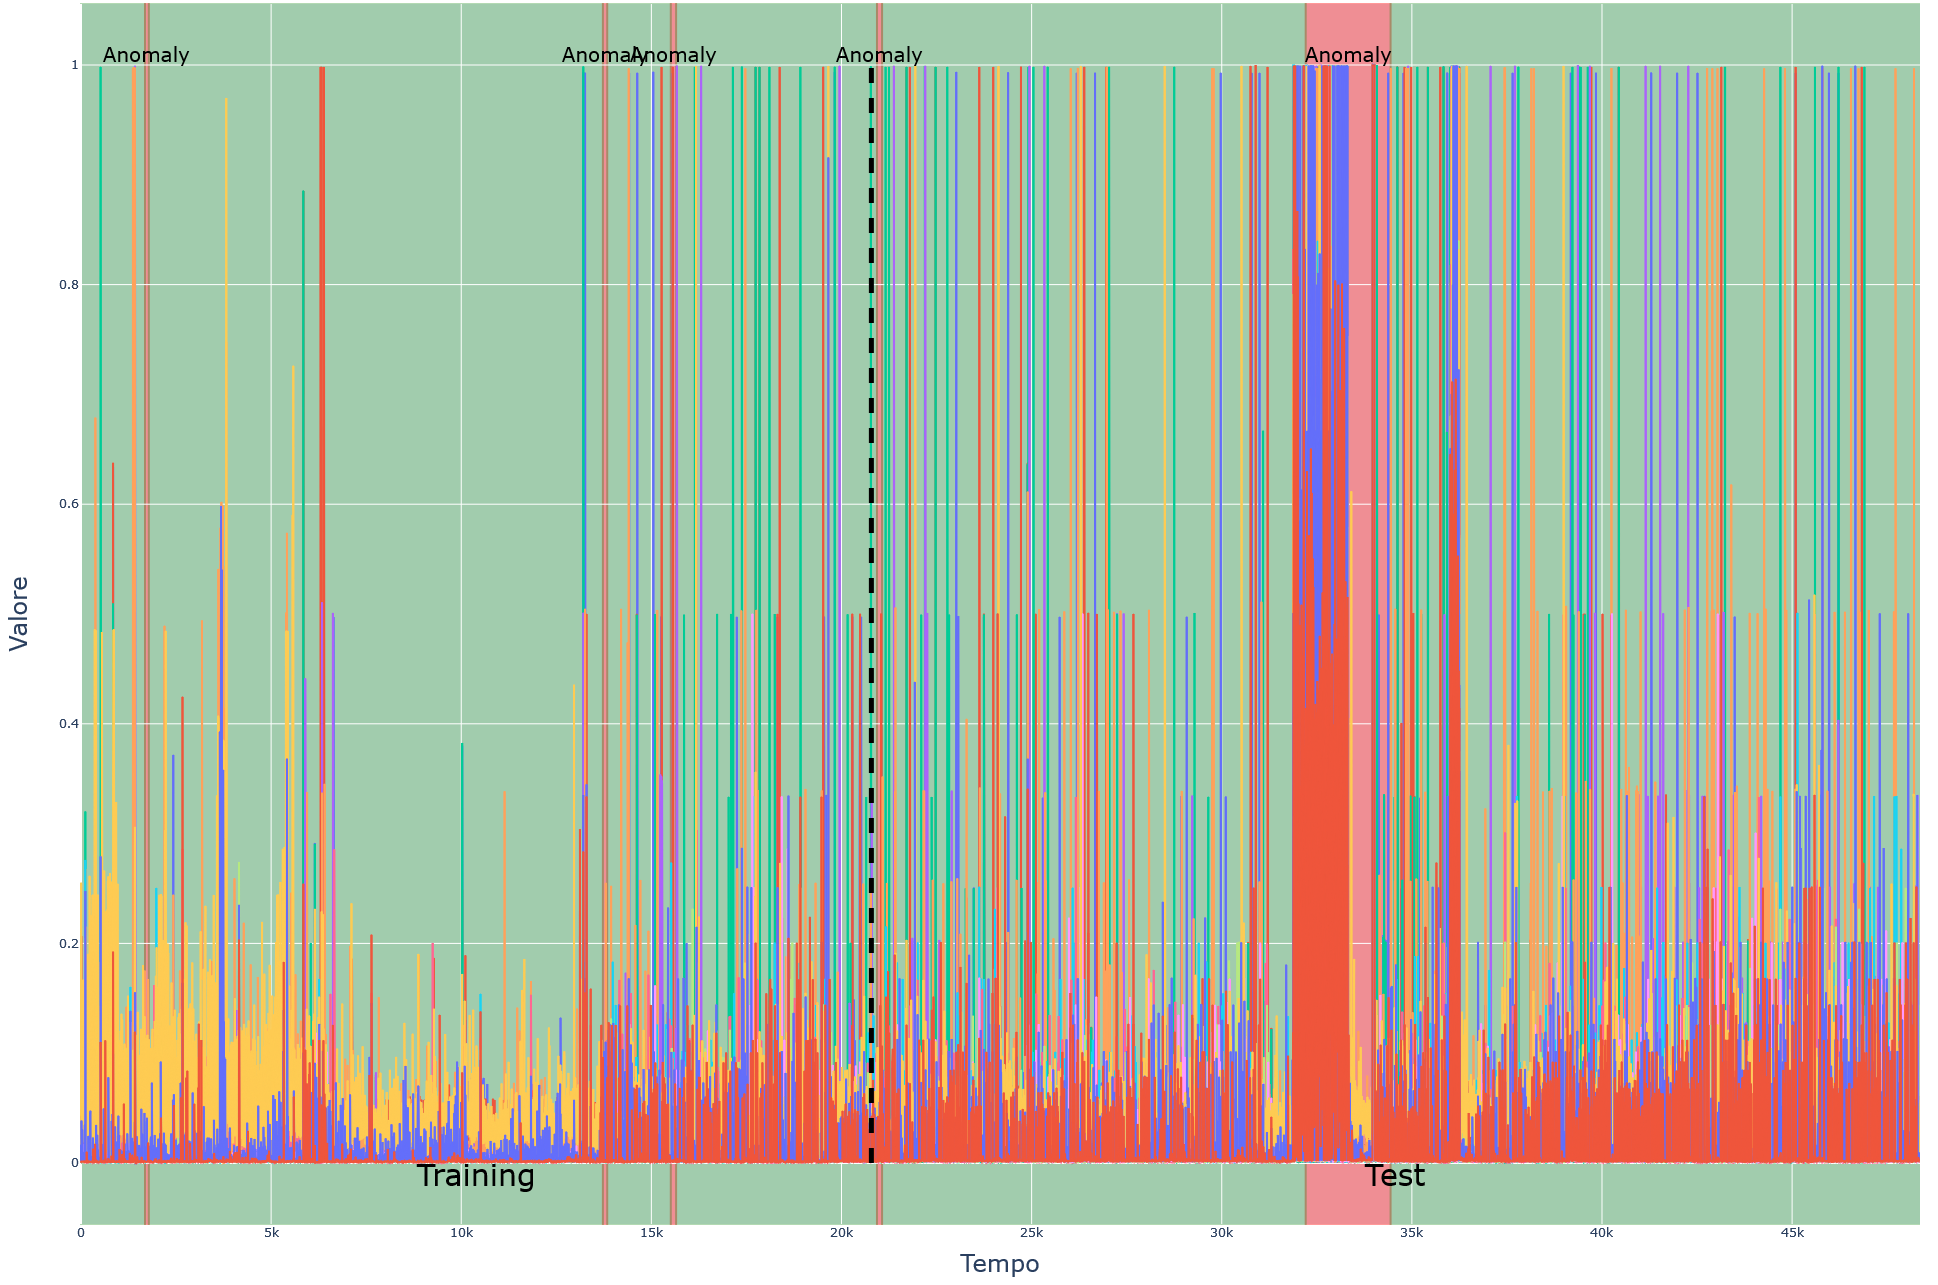
\includegraphics[width=0.6\textwidth]{./input/chapters/models/figs/telemanom-data.png}
        \caption{Suddivisione dataset negli insiemi di training e test. La linea tratteggiata delimita il dataset 
        di training da quello dedicato al test.}
        \label{fig:telemanom-data}
    \end{figure}

    \begin{figure}[H]
        \centering
        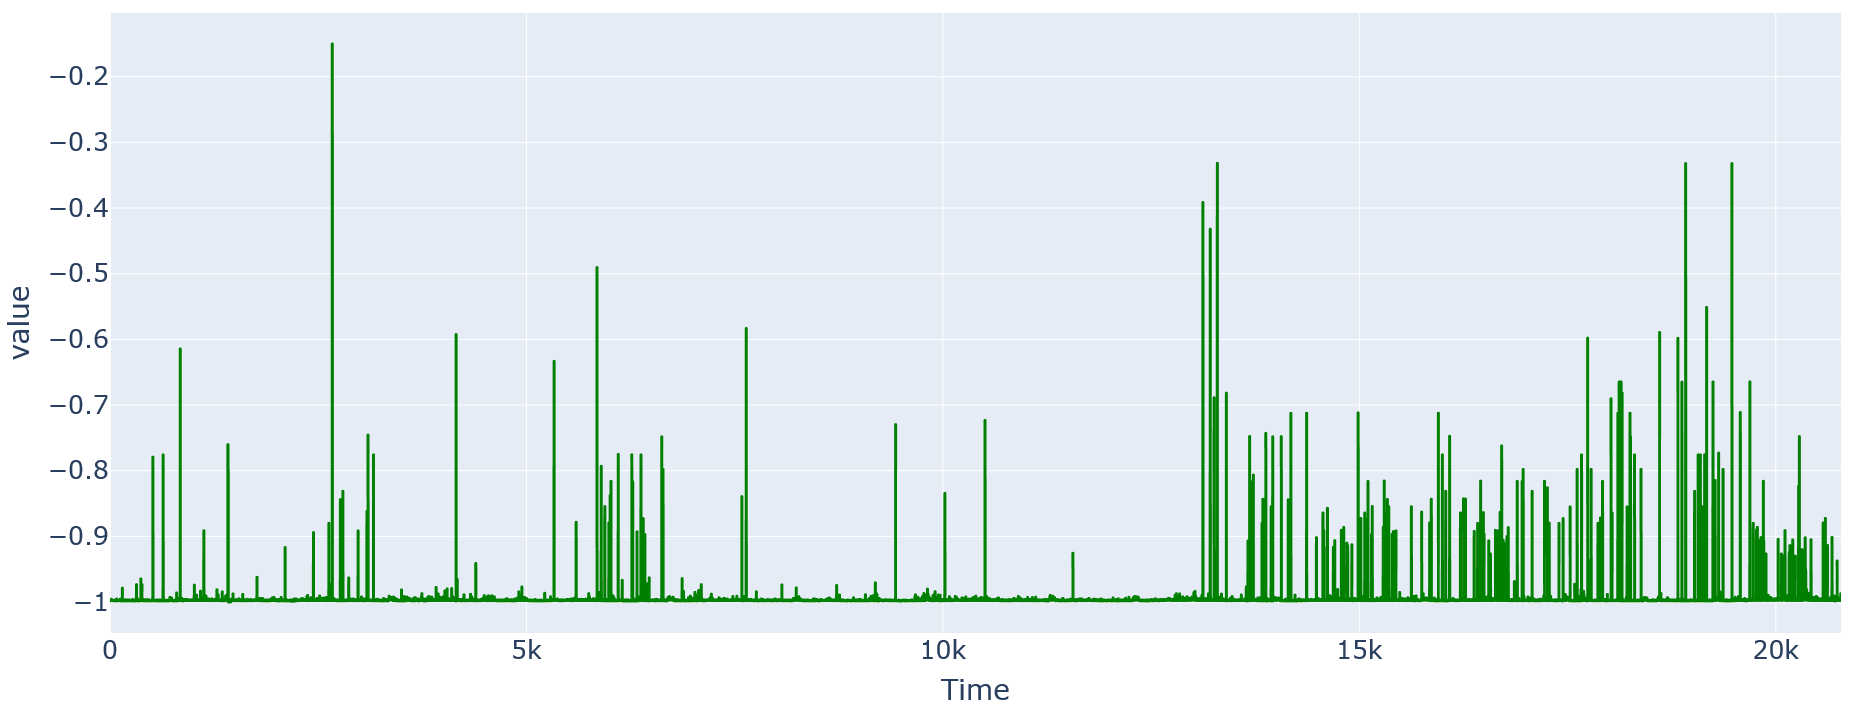
\includegraphics[width=0.7\textwidth]{./input/chapters/models/figs/telemanom-train-data.png}
        \caption{Insieme di training di Telemanom.}
        \label{fig:telemanom-train}
    \end{figure}

    Non è stato necessario assicurare una parte di dati al validation set perché Telemanom, nella sua 
    implementazione, gestisce da sé la validazione per l'addestramento della sua rete neurale.

    \paragraph{Iperparametri} Telemanom presenta numerosi iperparametri, tra i quali i più significativi sono riportati nella
    \hyperref[tab:telemanom-hyperparams]{Tabella 3.5.}, insieme ai valori empiricamente scelti per questo esperimento.
        
    \begin{table}[H]
        \centering
        \caption{Descrizione e valori degli iperparametri Telemanom.}
        \begin{tabular}{p{0.25\linewidth}p{0.55\linewidth}p{0.10\linewidth}}
            \toprule
            \textbf{Iperparametro} & \textbf{Informazioni} & \textbf{Valore}\\
            \toprule
            $batch\_size$ & Indica il numero di valori da considerare in ogni batch durante l'addestramento. & $100$\\
            \midrule
            $window\_size$ & Specifica il numero di batch precedenti da utilizzare nel calcolo dell'errore smussato.  & $110$\\
            \midrule
            $smoothing\_perch$ & Determina l'indice di smussamento nel calcolo degli errori. & $0.1$ \\
            \midrule
            $layers$ & Vettore bidimensionale che rappresenta il numero di neuroni negli strati nascosti della rete neurale. & $[100,100]$\\
            \midrule
            $l_s$ & Numero di passi temporali precedenti a quello attuale su cui verrà basata la previsione futura. & $7$ \\
            \midrule
            $n\_predictions$ & Indica il numero di valori futuri da prevedere. & $35$ \\
            \midrule
            $validation\_split$ & Specifica la percentuale del dataset di training che verrà usato come validazione per l'addestramento 
                della rete neurale. & $0.2$\\
            \bottomrule
        \end{tabular}
        \label{tab:telemanom-hyperparams}
    \end{table}


        % !TEX root = ../thesis.tex
    
%**************************************************************
% MSCRED
%**************************************************************

\subsection{Multi-Scale Convolutional Recurrent Encoder-Decoder}
    MSCRED\cite{mscred} è un recente modello avanzato che si concentra sull'identificazione di anomalie all'interno di serie 
    temporali multivariate.

    \paragraph{Scelta del modello} MSCRED è stato scelto per diverse ragioni; come attestano gli autori del paper,
    è in grado di catturare informazioni a diverse scale temporali, grazie all'incorporazione di strati convoluzionali. 
    Inoltre, la sua architettura di codifica-decodifica è adatta per l'identificazione di pattern complessi. Fondamentalmente, 
    il modello è stato sviluppato con l'obiettivo specifico di gestire l'intercorrelazione dei segnali e la 
    dipendenza temporale tra di essi. Lo scopo principale è valutare se questo approccio avanzato possa migliorare 
    significativamente il rilevamento delle anomalie rispetto a modelli più tradizionali come 
    ARMA\cite{arma} e OC-SVM\cite{ocsvm}.
    
    
    \paragraph{Le controversie sul modello} L'implementazione originale, disponibile su 
    GitHub\footnote{\url{https://github.com/7fantasysz/MSCRED}}, non è stata accolta con entusiasmo dalla critica online. 
    Purtroppo, di per sé, il codice non è molto intuibile e sono presenti 
    dei riferimenti agli ambienti locali dello sviluppatore originale. Inoltre, nell'implementazione originale, le etichette
    che rappresentano le anomalie nel dataset non sono state fornite, rendendo impossibile replicare i risultati del paper.
    Tutto questo ha fatto suscitare dubbi riguardo all'effettiva efficacia del modello. Nella repository 
    GitHub\footnote{\url{https://github.com/Pikarz/tirocinio\_infostud}} relativa agli studi affrontati in questa relazione viene 
    allegata la versione del codice revisionata e rinnovata a fondo dal sottoscritto con cui sono stati effettuati gli esperimenti.


    \paragraph{Il framework del modello}
    Per quanto riguarda il modello in sé, le "signature matrices" sono una parte fondamentale di MSCRED e svolgono un 
    ruolo chiave nell'analisi delle serie temporali. Queste matrici sono utilizzate per rappresentare le intercorrelazioni
    tra diverse coppie di serie temporali in un segmento specifico della serie, una proprietà critica che riflette lo
    stato del sistema.
    

    Le signature matrices sono matrici $n \times n$ dove $n$ è il numero di segnali della serie temporale analizzata.
    Una certa signature matrix $M^t$ è costruita attraverso il prodotto interno di due serie temporali all'interno del segmento 
    interessato. Formalmente, date due serie temporali $\mathbf{x}^w_i = (x^{t-w}_i, x^{t-w-1}_i, \dots, x_i^t)$ e $\mathbf{x}_j^w =
    (x_j^{t-w}, x_j^{t-w-1}, \dots, x_j^t)$ appartenenti allo stesso segmento $X^w$, la loro correlazione $m_{ij}^t \in M^t$ è 
    calcolata secondo l'\hyperref[eq:sign-matr]{equazione 3.3.}

    \begin{equation}\label{eq:sign-matr}
        m_{ij}^t =\frac{\sum_{\delta=0}^w x_i^{t-\delta}x_j^{t-\delta}}{w}
    \end{equation}
            
    \begin{figure}[H]
        \centering
        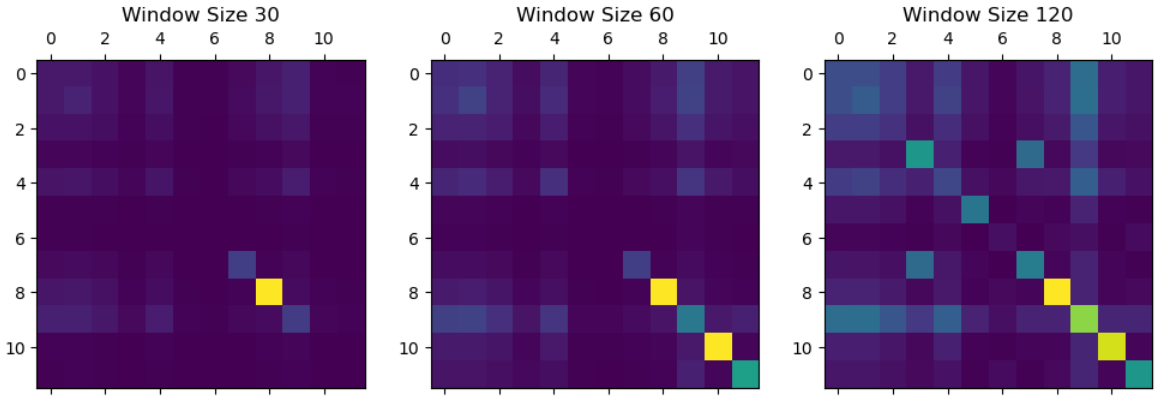
\includegraphics[width=0.6\textwidth]{./input/chapters/models/figs/signature_matrices.png}
        \caption{Signature matrices.} % Use caption to create a caption
        \label{fig:signature-matrices}
    \end{figure}

    Banalmente, le signature matrices sono matrici simmetriche. Nell'esperimento, l'intervallo tra due segmenti è 
    $gap\_time = 30$ e vengono costruite $s=3$ signature matrices con grandezze diverse pari a $win\_sizes = [30, 60, 120]$ punti
    temporali.
    Nella \hyperref[fig:signature-matrices]{Figura 3.8.} è illustrato un esempio di tre signature matrices su cui si
    basano i risultati dell'esperimento riportati nella \hyperref[val-mscred]{Sezione 4.5}.

    In sintesi, le signature matrices vengono concatenate e il tensore risultante $\chi^{t,0} \in \mathbb{R}^{n \times n \times s}$ 
    viene fornito in input a vari strati convoluzionali. Sia $\chi^{t,l}$ la feature map del livello $l$-esimo, attraverso un 
    attention based ConvLSTM\cite{convlstm} vengono aggiornati gli strati nascosti delle feature map $\mathcal{H}^{t,l}$ in $\hat{\mathcal{H}}^{t,l}$. 
    In seguito, attraverso un decodificatore convoluzionale, le feature map ottenute al passo precedente vengono decodificate e
    vengono ricostruite le signature matrices facendo, essenzialmente, il processo inverso: la feature map $\hat{\mathcal{H}}^{t,l}$ 
    viene data in input a una rete neurale deconvoluzionale e l'output, la feature map $\hat{\chi}^{t,l}$, è concatenato 
    con l'output del precedente layer convoluzionale. La concatenazione è poi data in input al prossimo strato deconvoluzionale. 
    L'output finale $\hat{\chi}^{t,0}$ denota le signature matrices ricostruite. La funzione di loss di MSCRED, osservabile
    nell'\hyperref[eq:mscred-loss]{equazione 3.4}, osserva la differenza tra le signature matrices originali e quelle ricostruite e, 
    nel corso delle epoche di training, punta a minimizzare tale funzione di loss.       

    \begin{equation}\label{eq:mscred-loss}
        \mathcal{L}_{MSCRED} = \sum_t \sum_{c=1}^s \Vert \chi^{t,0}_{:,:,c} - \hat{\chi}^{t,0}_{:,:,c} \Vert^2_F
    \end{equation}



    \paragraph{Il dataset} La suddivisione del dataset negli insiemi di training, validazione e test ha mantenuto 
    gli indici di suddivisione usati nell'esperimento di OC-SVM, osservabile nella 
    \hyperref[tab:dataset-ocsvm]{Tabella 3.2.}

    \paragraph{Iperparametri} MSCRED, come già anticipato nei paragrafi precedenti, presenta diversi iperparametri, tra cui 
    $win\_sizes$ che rappresenta la larghezza delle signature matrices, $gap\_time$, che determina la distanza tra i segmenti 
    della serie temporale, ovvero identifica quanto scorre ogni finestra a ogni passo, e $s$ che è il numero signature matrices. 
    Inoltre, l'iperparametro $step\_max$ rappresenta il numero di feature maps precedenti 
    concatenate dal codificatore convoluzionale e $thred\_b$ e $threshold$ regolano la sensibilità del modello 
    nel determinare le anomalie. In particolare, $thred\_b$ rappresenta un valore di soglia specifico utilizzato 
    dal modello per valutare numericamente l'indice di anomalia degli elementi all'interno dei dati, associando a essi
    un certo punteggio di anomalia. $threshold$, invece, è atto a valutare le prestazioni complessive 
    del modello e stabilisce una soglia oltre la quale i punteggi di anomalia vengono etichettati come anomalie.

    Dopo un'attenta analisi sono stati scelti per l'esperimento gli iperparametri riportati nella 
    \hyperref[tab:mscred-iperparams]{Tabella 3.6.} che hanno garantito la migliore soluzione
    empirica. I restanti iperparametri $thred\_b$ e $threshold$, sono stati ottimizzati tramite una grid-search atta 
    a massimizzare la metrica F1.

    \begin{table}[H]
        \centering
        \caption{Iperparametri MSCRED (parte 1.)}
        \begin{tabular}{lc}
            \toprule
            \textbf{Iperparametro} & \textbf{Valore} \\
            \toprule
            $win\_sizes$ & $30, 60, 120$ \\
            $s$ & $3$ \\
            $step\_max$ & $20$ \\
            $gap\_time$ & $30$ \\
            \bottomrule
        \end{tabular}
        \label{tab:mscred-iperparams}
    \end{table}

    Formalmente, siano $\mathbf{Tr}, \mathbf{Va}$ i dataset utilizzati per il training e
    per il validation rispettivamente, e sia $\text{MSCRED}_\mathbf{X}^\mathbf{Y}$ un modello MSCRED addestrato con gli iperparametri 
    della \hyperref[tab:mscred-iperparams]{Tabella 3.6.} su $\mathbf{X}$ che effettua previsioni nei punti $\mathbf{Y}$, 
    e sia $thred\_bs_{50}$ uno spazio lineare costituito da elementi equidistanti $thred\_b_i$ tali che $thred\_b_i \in 
    [1\mathrm{e}{-11}, 1\mathrm{e}{-6}] \forall i \in [50]$ e sia 
    $Thres$ la lista esaustiva dei possibili threshold, ovvero dei vari anomaly score $V_{\text{score}}$, 
    generati dal modello per ogni punto:

    \begin{equation}
        \label{eq:mscred-problem}
        \begin{aligned}
            & thred\_b^*, threshold^* = \max_{\substack{thred\_b, \\ threshold}} F1(\text{MSCRED}_\mathbf{Tr}^\mathbf{Va}(thred\_b, threshold)) \\
            & \text{con il vincolo} \quad thred\_b \in thred\_bs_{50}, threshold \in V_{\text{score}}
        \end{aligned}
    \end{equation}

    \begin{table}[H]
        \centering
        \caption{Iperparametri MSCRED (parte 2.)}
        \begin{tabular}{lc}
            \toprule
            \textbf{Iperparametro} & \textbf{Valore} \\
            \toprule
            $thred\_b^*$ & $6.326$ \\
            $threshold^*$ & $134.747$ \\
            \bottomrule
        \end{tabular}
        \label{tab:mscred-iperparams2}
    \end{table}
    Gli iperparametri che hanno soddisfatto l'\hyperref[eq:mscred-problem]{equazione 3.5} sono riportati nella 
    \hyperref[tab:mscred-iperparams2]{Tabella 3.7.}

    È bene notare che un numero di passaggi temporali pari a $gap\_time$ vengono collassati in uno singolo dopo la computazione di MSCRED,
    quindi data una serie temporale che contiene $x$ osservazioni, la soluzione generata avrà $x \bmod gap\_time$ osservazioni.